% !TeX root = bachelorarbeit.tex
\subsection{Referenzzelle und Hybridisierung}
\label{Referenzzelle&Hyb}
\subsubsection{Referenzzelle}
Bevor wie uns an dieser Stelle der Hybridisierung widmen können, wollen wir noch kurz auf einen wichtigen Aspekt der Implementierung finiter Elemente eingehen.
An dieser Stelle hat es sich bereits oft als nützlich erwiesen, eine sogenannte Referenzzelle einzuführen. Statt sich die Daten jeder Zelle statisch zu speichern und dann darauf zuzugreifen, gehen wir dabei stets von der Referenzzelle aus und können über je eine linear affine Abbildung in den tatsächlichen Zellen operieren. Da wir ausschließlich Vierecke verwenden, wollen wir uns dementsprechend an dieser Stelle auf Vierecke beschränken.

\begin{Definition}
	
	Das Referenzviereck $ \square $ ist definiert als
	\[ \hat{K} \coloneqq \conv \{ \hat{\mathcal{V}} \} \text{, wobei } \hat{\mathcal{V}} \coloneqq \left\{ 
	\begin{pmatrix}
	0\\
	0
	\end{pmatrix},
	\begin{pmatrix}
	1\\
	0
	\end{pmatrix},
	\begin{pmatrix}
	0\\
	1
	\end{pmatrix},
		\begin{pmatrix}
	1\\
	1
	\end{pmatrix} \right\} \]
	Die Seiten von $ \square $ sind
	\begin{align*}
	\hat{F}_0 &\coloneqq \conv \left\{ 
	\begin{pmatrix}
	0\\
	0
	\end{pmatrix},
	\begin{pmatrix}
	1\\
	0
	\end{pmatrix} \right\}\\
	\hat{F}_1 &\coloneqq \conv \left\{ 
	\begin{pmatrix}
	1\\
	0
	\end{pmatrix},
	\begin{pmatrix}
	1\\
	1
	\end{pmatrix} \right\}\\
	\hat{F}_2 &\coloneqq \conv \left\{ 
	\begin{pmatrix}
	1\\
	1
	\end{pmatrix},
	\begin{pmatrix}
	0\\
	1
	\end{pmatrix}
	 \right\}\\ 
	 \hat{F}_3 &\coloneqq \conv \left\{ 
	 \begin{pmatrix}
	 0\\
	 1
	 \end{pmatrix},
	 \begin{pmatrix}
	 0\\
	 0	
	 \end{pmatrix}
	 \right\}\\ 	
	\end{align*}
	Weiter sei $ \{ \hat{\psi}_i \}_{i=0}^3 $ die Seitenbasis aus Hütchenfunktionen
%	\begin{align*}
%	\hat{\psi}_0:\hat{K} \to \R^2, \hat{\psi}_0(\xi) &\coloneqq 
%	\begin{pmatrix}
%	\xi_1\\
%	\xi_2-1
%	\end{pmatrix}\\
%	\hat{\psi}_1:\hat{K} \to \R^2, \hat{\psi}_1(\xi) &\coloneqq  
%	\begin{pmatrix}
%	\xi_1\\
%	\xi_2
%	\end{pmatrix}\\
%	\hat{\psi}_2:\hat{K} \to \R^2, \hat{\psi}_2(\xi) &\coloneqq 
%	\begin{pmatrix}
%	\xi_1-1\\
%	\xi_2
%	\end{pmatrix}\\
%	\hat{\psi}_3:\hat{K} \to \R^2, \hat{\psi}_3(\xi) &\coloneqq 
%	\begin{pmatrix}
%	\xi_1-1\\
%	\xi_2
%	\end{pmatrix}.
%	\end{align*}
	und $ \hat{\nu} $ sei der äußere Normalenvektor von $ \hat{K} $.
\end{Definition}

\begin{figure}[H]
	\centering
	\captionabove{Referenzzelle}
	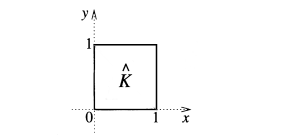
\includegraphics[width=0.33\textwidth]{referenzzelle2.png} \\
	Abbildung modifiziert aus \cite{knabner2013numerik} Seite 51
\end{figure}

\begin{Bemerkung}
	$\forall i,j\in\{0,1,2,3\} \colon \int_{F_j} \hat{\psi}_i \cdot \hat{\nu} \da = \delta_{i,j} \text{ und } \hat{\psi}_i \in \mathbb{P}_1(\hat{K}, \R^2).$
\end{Bemerkung}

Weiter setzen wir noch 
\begin{align*}
\text{ die Menge der Seiten }&& \hat{\mathcal{F}} &\coloneqq \left\{ \hat{F}_0, \hat{F}_1, \hat{F}_2,\hat{F}_3 \right\} \\
\text{und den Seitenansatzraum }&&  \hat{W} &\coloneqq \spann \left\{ \psi_0,\psi_1, \psi_2, \psi_3 \right\}.
\end{align*}
\textbf{Transformation von $ \hat{K} $ zu $ K $:} Für ein beliebiges $ K \in \mathcal{K} $ wollen wir jetzt eine Seitenbasis $ \{ \psi_0^K, \psi_1^K, \psi_2^K, \psi_3^K \} $ berechnen (Wie bisher gegeben durch $ \forall i\in\{0,1,2,3\}\colon \psi_i^K\in\mathbb{P}_1(K,\R^2) \text{ und } \int_{F_j^K} \psi_i^K \cdot \nu^K \da = \delta_{i,j} $, wobei $ \nu^K $ äußere Normale von  $ K $ und $ F_j^K  $ beliebige Seite von $ K $). Dazu betrachten wir die affine Transformationsabbildung $ \varphi_K $ von $ \hat{K} $ zu $ K $:
\begin{align*}
\varphi_K\colon \hat{K} \to K, \varphi_K(\xi) = z_{0,K} + B_K \xi \text{ mit passenden } B_K\in\R^{2 \times 2} \text{ und } \\
J_K \coloneqq \det(B_K) > 0.
\end{align*}

\begin{figure}[H]
	\centering
	\captionabove{Affine lineare Transformation von $\hat{K}$ nach $ K $}
	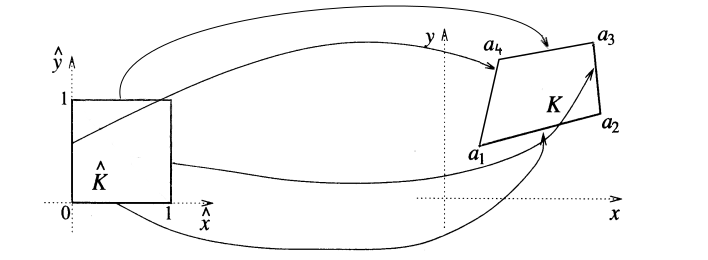
\includegraphics[width=0.55\textwidth]{affinlinearetransf2.png} \\
	Abbildung modifiziert aus \cite{knabner2013numerik} Seite 53
\end{figure} 
\begin{Lemma}
	Es gilt: $\nu^K = \frac{1}{\abs{B_K^{-T} \hat{\nu}}} B_K^{-T} \hat{\nu} $ ist Normale zu $ \partial K $.
\end{Lemma} $\newline$
Die Seitenbasis auf $ K $ ist dann gegeben durch 
\[ \psi_i^K = J_K^{-1}B_K \hat{\psi}_i \circ \varphi_K \ (i\in \{0,1,2,3\}) \]
Die globale Seitenbasis $\{\psi_j\}_{j = 1}^{\abs{\mathcal{F}}}$ auf $ \mathcal{D}  $ erhalten wir dann mithilfe einer weiteren Abbildung $l$, die zwischen der Seitennummerierung in einer Zelle $ K $ und der globalen Seitennummerierung vermittelt. Es ist dabei
\[ l\colon \mathcal{K}\times \{0,1,2,3\} \to \{1, \dots , \abs{\mathcal{F}} \}, (K,i) \mapsto l(K,i). \]
Wir setzen nun also $ \psi_j (j \in \{1,\dots , \abs{\mathcal{F}}\})$ durch
\[ \psi_j(x) = 
\begin{cases}
\psi_i^K(x) , &\text{falls } j = l(K,i)\\
0,			  &\text{sonst}.
\end{cases} \]
\begin{Bemerkung}
	Für alle Zellen $ K \in \mathcal{K} $ von denen $ F_j $ eine anliegende Seite ($ \overline{K} \cap F_j \ne \emptyset $) und $ F_j $ lokal mit $ i \in \{0,1,2,3\} $ nummeriert ist, gilt:
	\[ \psi_j|_K = \psi_i^K. \]
\end{Bemerkung}

\subsubsection{Hybridisierung}

Wir betrachten die Räume
\[W_K \coloneqq \left\{ \psi_K\colon K \to \R^2 \colon \psi_K = J_K^{-1}  B_K \hat{\psi} \circ \varphi_K^{-1}, \hat{\psi} \in \hat{W} \right\} \]
\[ W_\mathcal{K} \coloneqq \prod_{K \in \mathcal{K}} W_K, \qquad M_h \coloneqq \prod_{F \in \mathcal{F}} \mathbb{P}_0(F) \]
\[ M_h(u_D) \coloneqq \left\{ \mu_h \in M_h \colon \forall  F \subset \Gamma_D \int_F \mu_h \da = \int_F u_D \da  \right\}\]

An dieser Stelle nutzen wir die folgende Äquivalenz:\\
	\[ \psi_h \in W_h \iff \big[ \psi_h \in W_{\mathcal{K}} \text{ und }  (\psi_{K_1} - \psi_{K_2}) \cdot \nu^F = 0 \ (F= \partial K_1 \cap \partial K_2 \in \mathcal{F}^{\circ})\big] \]



Und untersuchen folgendes Problem:
\begin{align*}
\text{Bestimmme } (q_h,u_h, \lambda_h) \in W_\mathcal{K} \times \mathcal{Q}_h \times M_h(u_D) \text{ mit}\\
\begin{dcases}
(1) \int_K \kappa^{-1} q_h \psi_K \dx - \int_K u_h \dive(\psi_K) \dx = - \int_{\partial K} \lambda_h \psi_K \cdot \nu^K \da \\
(2) \int_K \dive(q_h) \phi_K \dx = 0\\
(3) \sum_{K\in \mathcal{K}} \int_{\partial K} q_h \cdot \nu \mu_h \da = - \int_{\Gamma_N} g_N \mu_h \da
\end{dcases}\\
\text{für alle } K \in \mathcal{K}, \psi_K \in W_K, \phi_K \in \mathcal{Q}_h  \text{ und } \mu_h \in M_h(0)
\end{align*}

Dieses Problem ist äquivalent zu dem diskreten gemischten FE-Problem, welches wir zuvor betrachtet haben:
\begin{align*}
\text{Bestimme } (q_h,u_h) \in W_h(-g_N) \times \mathcal{Q}_h \text{ mit}\\
\begin{cases}
\int_{\Omega} \kappa ^{-1} q_h \cdot \psi_h \dx \mkern-15mu &- \int_{\Omega} u_h \dive(\psi_h) \dx = - \int_{\Gamma_D} u_D \psi_h \cdot \nu \da\\
&- \int_{\Omega} \dive(q_h) \phi_h \dx = 0
\end{cases} \\
\text{für alle } (\psi_h, \phi_h) \in W_h(0) \times \mathcal{Q}_h
\end{align*}

Für ein festes $ K \in \mathcal{K} $ ergibt sich mit der Wahl einer Basis von $ W_K $, $ \mathcal{Q}_h $ und $ M_h $ 
%\begin{align*}
%	&W_K = \spann\{\psi_F \mid F \in \mathcal{F}_K \}  &&(\psi_F \cdot n^F)_{|F'} = \begin{cases}
%		1 &F = F'\\
%		0 &\text{sonst}
%	\end{cases}\\
%	&Q_h = \spann\{\eta_K \mid K \in \mathcal{K}  \}  &&{\eta_K}_{|K'} = \begin{cases}
%	1 &, K = K'\\
%	0 &,\text{sonst}
%	\end{cases}\\
%	&M_h = \spann \{ \nu_F \mid F \in \mathcal{F}_K \}  &&{\nu_F}_{|F'} = \begin{cases}
%		1 &, F = F'\\
%		0 &, \text{sonst}
%	\end{cases}  
%\end{align*}

eine Formulierung als LGS mit Nebenbedingung, wobei $ \ubar{q}_K \coloneqq \ubar{R}_K \ubar{q}, \ \ubar{u}_K \coloneqq \ubar{R}_K \ubar{u} $ .
\begin{align*}
\text{Bestimme } \ubar{q}, \ubar{u} \text{ und } \ubar{\lambda} \text{ mit}\\
\begin{dcases}
(1) \begin{pmatrix}
\ubar{A}_K & \ubar{B}_K \\
\ubar{B}_K^T & 0
\end{pmatrix}
\begin{pmatrix}
\ubar{q}_K\\
\ubar{u}_K
\end{pmatrix}
\mkern-16mu&= \begin{pmatrix}
- \ubar{C}_K \, \ubar{R}_K \ubar{\lambda} \\
0
\end{pmatrix}\\
(2) \sum_{K \in \mathcal{K}}  (\ubar{R}_K \ubar{\mu})^T \ubar{C}_K \ubar{q}_K \mkern-16mu&= \ubar{\mu}^T \ubar{b}		
\end{dcases}\\
\text{für alle } \ubar{\mu} \text{ mit } \ubar{\mu}[F] = 0 \text{ für } F \in \Gamma_D \cap \mathcal{F}
\end{align*}

\begin{align*}
\left(
\begin{array}{c}
1\\ 1 \\ \vdots \\ 1 \\ 1\\ \ubar{\mu}
\end{array}
\right)^T
\underbrace{\left(
	\begin{array}{ccccc|c}
	\ubar{A}_{K_1} & \ubar{B}_{K_1}&&&& \ubar{C}_{K_1} \ubar{R}_{K_1}\\
	\ubar{B}_{K_1} & 0 &&&& 0\\
	&& \ubar{A}_{K_2} & \ubar{B}_{K_2} && \ubar{C}_{K_2} \ubar{R}_{K_2}\\
	&  & \ubar{B}_{K_2} & 0 && 0\\
	&  &  &  &\ddots &\\
	\hline
	\ubar{R}_{K_1}^T \ubar{C}_{K_1}^T& 0 & \ubar{R}_{K_2}^T \ubar{C}_{K_2}^T& 0& &0 \\
	\end{array}
	\right)}_{\eqqcolon \left( \begin{array}{c|c}
	\ubar{D} & \ubar{E}\\
	\hline
	\ubar{E}^T & 0
	\end{array} \right)}
\underbrace{\left(
	\begin{array}{c}
	\ubar{q}_{K_1}\\ \ubar{u}_{K_1} \\ \ubar{q}_{K_2}\\ \ubar{u}_{K_2} \\ \vdots \\ \ubar{\lambda}
	\end{array}
	\right)}_{\eqqcolon \left( \begin{array}{c}
	\left(
	\begin{array}{c}
	\ubar{q}_{K_i}\\ \ubar{u}_{K_i}
	\end{array}
	\right)_{K_i \in \mathcal{K}} \\ \ubar{\lambda} 
	\end{array}\right)} = 
\left(
\begin{array}{c}
0\\ 0 \\ \vdots \\ 0 \\ 0\\ \ubar{\mu}^T \ubar{b}
\end{array}
\right)
\end{align*}
Mit dem Schurkomplement $ \ubar{S} \coloneqq \ubar{E}^T \ubar{D}^{-1} \ubar{E} $ folgt
\[ \ubar{\mu}^T \ubar{S} \, \ubar{\lambda} = \ubar{\mu}^T \ubar{b} 	\text{ für alle } \ubar{\mu} \text{ mit } \ubar{\mu}[F] = 0 \text{ für } F \in \Gamma_D \cap \mathcal{F} \]

Sobald wir $ \ubar{\lambda}_k \coloneqq \ubar{R}_K \ubar{\lambda}$ bestimmt haben, können wir auch das obere LGS (1) lösen, um $ \ubar{q}_K $ und $ \ubar{u}_K $ zu erhalten.
% Um $ \ubar{\lambda}_k $ zu erhalten lösen wir das globales System:
%\begin{align*}
%	\underline{S} \, \underline{\lambda} = \underline{b}
%\end{align*}
%und bekommen somit $ \ubar{\lambda}_k $ über die Restriktionen
%\[ \ubar{\lambda} = \sum_{K \in \mathcal{K}} \ubar{R}_K \ubar{\lambda}_K .\]
